\section{Experiment Flow}
We fit a model on the train dataset. Optimal parameters are chosen through cross-validation if needed. We analyze model robustness and calculate Mean Squared Error of prediction. \
\subsection{Expected tables and figures}
\begin{enumerate}
    \item Graph of model prediction and true target against complex index
    \item Histogram of relative error distribution
    \item Table with MSE depending on model parameters selection
\end{enumerate}
\subsection{Visualization}
The source dataset contains 2327 protein complexes. We provide following plots for better understanding of given input.
\begin{figure}[!ht]
  \subfloat{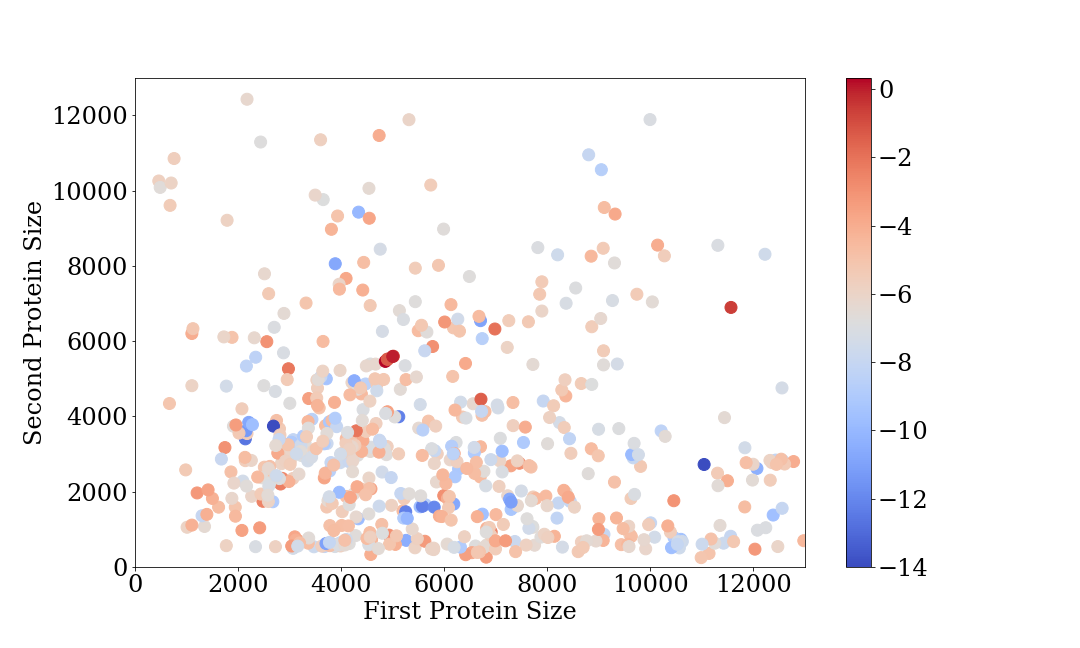
\includegraphics[width=0.5\textwidth]{contents/visual.png}}
  \subfloat{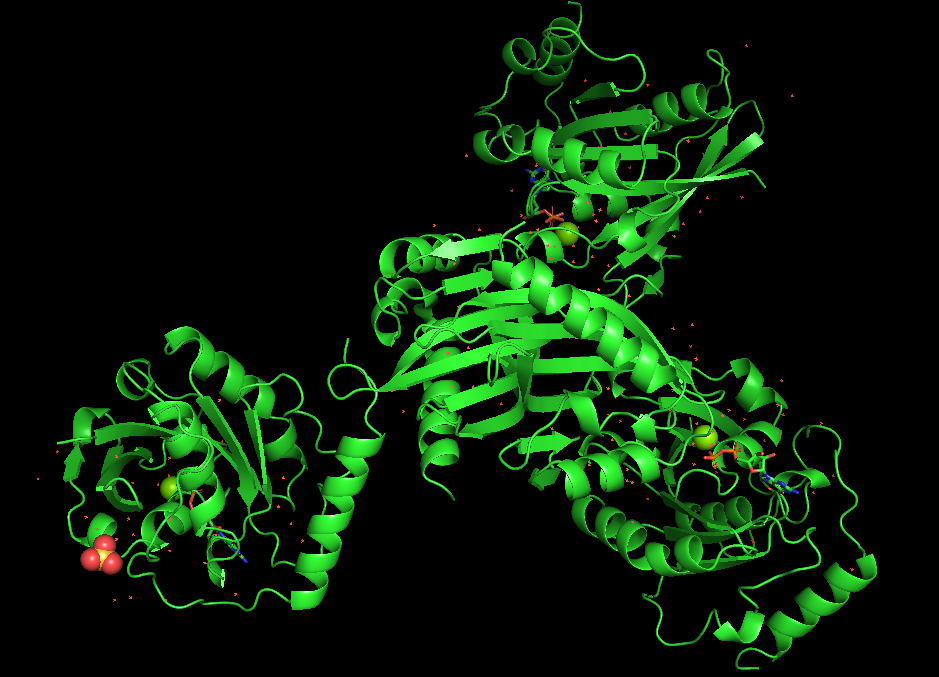
\includegraphics[width=0.5\textwidth]{contents/complex.png}}\\
 \caption{Source data target visualization / Example of source protein}
  \label{fig:3}
\end{figure}